\documentclass[conference]{IEEEtran}
\IEEEoverridecommandlockouts

% The preceding line is only needed to identify funding in the first footnote. If that is unneeded, please comment it out.
\usepackage{cite}
\usepackage{amsmath,amssymb,amsfonts}
\usepackage{algorithmic}
\usepackage{graphicx}
\usepackage{textcomp}
\usepackage{xcolor}
\def\BibTeX{{\rm B\kern-.05em{\sc i\kern-.025em b}\kern-.08em
    T\kern-.1667em\lower.7ex\hbox{E}\kern-.125emX}}

% -----
\usepackage{fontspec}
\usepackage{xltxtra}
\usepackage{xunicode}
\usepackage{scrextend}

% Thai Language setup
\XeTeXlinebreaklocale{'th'}
\newfontfamily\thaifont{TH Sarabun New}
\setmainfont{TH Sarabun New}
\changefontsizes[12pt]{12pt}
\XeTeXlinebreakskip = 0pt plus 1pt
\defaultfontfeatures{Scale=1.23}
% -----

\def\StudentId{63199130350}
\def\Me{นายสิทธิพงษ์ เหล่าโก้ก}
\def\MyEmail{sitdhibong.laokok@g.swu.ac.th}
\def\SNATopic{พฤติกรรมของผู้เรียนในระบบการเรียนออนไลน์ขนาดใหญ่ซึ่งนำไปสู่การยุติการเรียน}
\def\SNATopicEN{Behavior of Online Learner in MOOC Platform Leading to Course Drop-out}
\def\VirtualClassroom{ห้องเรียนเสมือน}
\def\moocs{การเรียนการสอนขนาดใหญ่}
\def\MOOCs{ระบบ{\moocs}}
\def\dropout{ยุติการเรียนกลางคัน}

\def\IEEEkeywordsname{คำสำคัญ}
\def\abstractname{บทคัดย่อ}
\def\figurename{รูปที่}

\title{
    \SNATopic \\
}
\author{
    \IEEEauthorblockN{\Me} \newline
    \IEEEauthorblockA{\MyEmail} \newline
    \IEEEauthorblockA{ภาคการศึกษาที่ 2 ประจำปีการศึกษา 2563} \newline
    \IEEEauthorblockA{ภาควิชาวิทยาการคอมพิวเตอร์ คณะวิทยาศาสตร์} \newline
    \IEEEauthorblockA{มหาวิทยาลัยศรีนครินทรวิโรฒ ประสานมิตร}
}

% Command
\newcommand{\thead}[1]{c}{\bfseries #1}

\begin{document}

    \maketitle

    \begin{abstract}
        Lorem ipsum
    \end{abstract}

    \begin{IEEEkeywords}
        MOOC, Learner Behavior, Online Course Dropout, Online Course Retired
    \end{IEEEkeywords}

    % = = = = = = = = = = = = = = =
    \section{บทนำ}
    เมื่อเกิดการระบาดของโคโรนาไวรัส (Coronavirus) ในช่วงปลายปี พ.ศ. 2562 \cite{covid:coronavirus}
    ที่แพร่ระบาดไปทั่วโลก และยังคงระบาดอย่างต่อเนื่องอยู่ในหลายประเทศทั่วโลก \cite{covid:worldtrendspread}
    รวมถึงในประเทศไทย \cite{covid:thailandspread} ที่เกิดการแพร่ระบาดเพิ่มมากขึ้นเรื่อยๆ
    ส่งผลให้เกิดมาตรการควบคุมกิจกรรมออกมา เพื่อลดการมีปฏิสัมพันธ์กันระหว่างบุคคล 
    และควบคุมสถานการณ์การระบาดของโคโรนาไวรัส \cite{covid:ratchakitcha:22}
    ทั้งนี้ ส่งผลให้หลายกิจกรรมนั้นจำเป็นต้องปรับเปลี่ยนการดำเนินกิจกรรมจากเดิม
    ให้สอดคล้องกับมาตรการควบคุม และคำแนะนำทางด้านสาธารณสุข \cite{covid:socialdistancing} 
    ทั้งการเพิ่มระยะห่างในการทำกิจกรรม การลดระยะเวลาการให้บริการ 
    ไปจนกระทั่งงดดำเนินการกิจกรรมหรือการให้บริการบางประเภทไป 
    และมาตรการควบคุม เพื่อลดการมีปฏิสัมพันธ์กันระหว่างงบุคล เว้นระยะห่างในกิจกรรมต่างๆ 

    ซึ่งกิจกรรมหนึ่งที่ได้รับผลกระทบตามมาด้วยนั่นก็คือกิจกรรมในสถานศึกษา 
    ที่ได้ปรับเปลี่ยนรูปแบบการดำเนินการจากการเรียนการสอนในห้องเรียน 
    ไปสู่รูปแบบการเรียนการสอนผ่านระบบการเรียนการสอนออนไลน์ หรือห้องเรียนเสมือน
    (Virtual Classroom) และสร้างปฏิสัมพันธ์กับชั้นผ่านแพลตฟอร์มการเรียนการสอนออนไลน์
    ที่สามารถรองรับการเรียนการสอนขนาดใหญ่ที่เรียกว่า MOOCs (Massive Open Online Courses)
    ซึ่งมีซอฟต์แวร์ที่มักจะนำมาใช้พัฒนาห้องเรียนเสมือน ได้แก่ Open edX \cite{mooctools:openedx},
    หรือ moodle \cite{mooctools:moodle} โดยที่การเรียนในรูปแบบห้องเรียนเสมือนเองนั้น
    ต่างก็มีปัจจัยหลายด้านประกอบเข้าด้วยกัน 
    ทั้งสภาพแวดล้อมของนักเรียนแต่ละคนที่ส่งผลต่อสมาธิการเรียน สิ่งเร้าภายนอก
    ประสิทธิภาพของอุปกรณ์ คอมพิวเตอร์ สัญญาอินเทอร์เน็ต 
    ทั้งหมดนี้อาจส่งผลต่อประสิทธิภาพการเรียนการสอนในรูปแบบห้องเรียนเสมือนได้ทั้งสิ้น
    ซึ่งในช่วงเวลาปรกตินั้น พบว่าผู้เรียนในหลักสูตรออนไลน์ในระบบการเรียนการสอนผ่าน
    MOOCs นั้นมีน้อยกว่า 5\% ที่ศึกษาจนเสร็จสิ้นหลักสูตรที่กำหนดไว้ในบทเรียน \cite{Feng_Tang_Liu_2019}
    หรือในอีกแง่หนึ่งก็คือ มีผู้เรียนมากว่า 95\% 
    ที่หยุดเรียนกลางคันก่อนที่จะศึกษาเนื้อหาจนกระทั่งจบหลักสูตร

    ซึ่งในช่วงเวลาที่จำเป็นจะต้องปรับรูปแบบการเรียนการสอน 
    ผ่านห้องเรียนเสมือนที่จัดทำการเรียนการสอนผ่านระบบออนไลน์ทั้งหมดแล้วนั้น
    ถึงแม้ว่า จะมีลักษณะการเรียนการสอนคล้ายคลึงกันกับการเรียนการสอนในห้องเรียนปรกติ
    ที่ผู้สอนนั้นยังคงติดตาม และกำหนดโครงสร้างกิจกรรมของชั้นเรียน 
    ซึ่งต่างจากการเรียนการสอนผ่านระบบการเรียนการสอนขนาดใหญ่ 
    ที่บางส่วนให้อิสระกับผู้เรียนในการศึกษาเนื้อหาในหลักสูตรที่กำหนดไว้อย่างเต็มที่ 
    แต่ก็เลี่ยงไม่ได้เลยว่า เนื้อหาบางส่วนนั้นจำเป็นจะต้องให้ผู้เรียนไปศึกษาเนื้อหานั้นด้วยตนเองตามที่กำหนด
    
    ดังนั้น จึงเป็นจุดสนใจในการศึกษาวิจัยที่ว่า หากสามารถเข้าใจลักษณะพฤติกรรมของผู้เรียน
    แล้วตรวจสอบได้ว่าผู้เรียนมีแนวโน้มที่จะละความสนใจจากเนื้อหาของหลักสูตร
    ก่อนที่เหตุการณ์นั้น ๆ จะเกิดขึ้นจริง เพื่อเพิ่มประสิทธิภาพในการเรียนการสอนผ่านห้องเรียนเสมือน
    โดยอาศัยการศึกษาข้อมูลพฤติกรรมร่วม (Collective Behavior) 
    \cite{mooc:collectivebehavior} ของผู้เรียนที่มีปฏิสัมพันธ์กับหลักสูตรใน{\MOOCs} 
    ซึ่งยุติการเรียนในหลักสูตรนั้นกลางคัน ก่อนสิ้นสุดการศึกษาตามเนื้อหาที่หลักสูตรกำหนดไว้

    % = = = = = = = = = = = = = = =
    \section{งานวิจัยที่เกี่ยวข้อง}

    เพื่อกำหนดแนวทางการศึกษาข้อมูล 
    จึงได้ค้นหาข้อมูลงานวิจัยที่เกี่ยวข้องเพื่อใช้วางแผนการวิจัยและพัฒนาต่อยอด 
    พบว่ามีงานวิจัยที่เกี่ยวข้องดังนี้

    \subsection{แนวทางการลดจำนวนการยุติการเรียนใน MOOCs: ด้วยแบบแผนการใช้ตัวแทนเป็นหลัก สำหรับการเรียนแบบมีส่วนร่วมบนพื้นฐานของระบบเครือข่ายสังคม \cite{paper:8924433}}
    lorem ipsum dolor sit amet

    \subsection{การค้นพบรูปแบบพฤติกรรมการเรียนเพื่อทำนายการยุติการเรียนใน MOOC \cite{paper:8085583}}
    lorem ipsum dolor sit amet

    \subsection{การทำนายการยุติการเรียนใน MOOCs ด้วยแนวคิดในรูปแบบ WCLSRT \cite{paper:9390886}}
    lorem ipsum dolor sit amet

    \subsection{การประยุกต์ใช้งานข้อมูลมหัตในภาคการศึกษา: การทำนายการยุติการเรียนใน MOOCs ที่ใช้ edX \cite{paper:7545065}}
    lorem ipsum dolor sit amet

    % = = = = = = = = = = = = = = =
    \section[technicalbackground]{วิธีการที่นำมาใช้งาน}

    ในกระบวนการศึกษาเพื่อทำความเข้าใจกับพฤติกรรมของผู้เรียนที่{\dropout}นั้น
    จะศึกษาชุดพฤติกรรมของผู้เรียนโดยใช้ชุดข้อมูลเปิดของมหาวิทยาลัยสแตนฟอร์ด 
    ซึ่งเป็นชุดข้อมูลเปิดเผย ที่จัดเก็บพฤติกรรมของพฤติกรรมของผู้เรียนใน{\MOOCs}
    จากนั้นจึงนำข้อมูลนี้มาจัดรูปแบบให้อยู่ในลักษณะของฐานข้อมูลกราฟ 
    แล้วจึงวิเคราะห์ข้อมูลพฤติกรรมด้วยวิธีการของกราฟเพื่อหาพฤติกรรมร่วม
    ของผู้เรียนที่{\dropout}ใน{\MOOCs} โดยมีขั้นตอนดังนี้

    \subsection[overview step]{ภาพรวมการทำงาน}

    เพื่อกำหนดกรอบการดำเนินงานในการวิจัยจึงได้กำหนดแนวทางการศึกษาข้อมูลไว้่
    โดยเริ่มต้นจากการ \textbf{ศึกษาชุดข้อมูล} ซึ่งเป็นเป็น \textbf{ชุดข้อมูลจาก Standford} 
    ที่จัดเก็บพฤติกรรมการเรียนของผู้เรียน ที่มีปฏิสัมพันธ์กับเนื้อหาของหลักสูตร 
    ซึ่งผลลัพธ์ที่ได้ออกมาจากขั้นตอนนี้จะเป็น \textbf{คุณลักษณะของข้อมูล} 
    เพื่อให้เข้าใจภาพรวมของข้อมูลและคุณลักษณะต่าง ๆ ของข้อมูลที่นำมาใช้ได้ 
    หลังจากนั้นจะ\textbf{นำข้อมูลเข้าสู่ฐานข้อมูลกราฟ}
    แล้วจึงกำหนดโครงสร้างกราฟตามคุณลักษณะของข้อมูลที่ทราบ 
    โดยจะได้\textbf{ฐานข้อมูลกราฟ}ออกมาในขั้นตอนนี้ 
    ซึ่งสามารถนำมาใช้\textbf{วิเคราะห์พฤติกรรมจากข้อมูลกราฟ}จากฐานข้อมูลที่ได้จากขั้นตอนก่อนหน้านี้
    โดยคาดว่าผลลัพธ์ที่ได้จะเป็น\textbf{ข้อมูลพฤติกรรมผู้เรียนที่{\dropout}} 
    ซึ่งผลการศึกษานี้ จะนำมา\textbf{สรุปผลการศึกษา} เป็น\textbf{ผลการศึกษา}ถัดไป
    ดังที่แสดงไว้ในรูปที่ \ref{fig:overview-process}
    \begin{figure}[htbp]
        \centering{
            \includegraphics[width=0.35\textwidth]{assets/Process-Outline}
        }
        \caption{กระบวนการทำงานโดยภาพรวมเพื่อศึกษาพฤติกรรมของผู้เรียน}
        \label{fig:overview-process}
    \end{figure}

    \subsection[datacharacteristics]{ลักษณะข้อมูล}
    ข้อมูลที่นำมาใช้ประกอบการศึกษานี้ได้มาจากข้อมูลพฤติกรรมของผู้เรียน ที่จัดเก็บจาก{\MOOCs} 
    ซึ่งเป็นชุดข้อมูลที่เปิดเผย ประกอบบทความวิชาการเรื่อง 
    \textit{"Predicting Dynamic Embedding Trajectory in Temporal Interaction Networks"} 
    \cite{DBLP:journals/corr/abs-1908-01207} ที่ได้ศึกษาลักษณะความสัมพันธ์ที่เกิดขึ้นชั่วคราวในเครือข่าย
    ด้วยชุดข้อมูลหลายประเภท ซึ่งพฤติกรรมการเรียนใน{\MOOCs}เป็นส่วนหนึ่งของบทความวิชาการนี้
    โดยข้อมูลที่ได้จะประกอบไปด้วย ข้อมูลผู้เรียน (Learner), การลงทะเบียน (Enrollment), 
    หลักสูตร (Course), โครงสร้างหลักสูตร ซึ่งประกอบไปด้วยส่วนประกอบ (Module) 
    และชิ้นส่วนย่อยของส่วนประกอบนั้น (Module Object), 
    ป้ายกำกับสถานะการเรียนของผู้ใช้งานในหลักสูตรนั้น ว่าเกิดการ{\dropout} ขึ้นหรือไม่
    และข้อมูลที่ผู้ใช้งานได้ปฏิสัมพันธ์กับเนื้อหาในหลักสูตร \cite{mooc:stanforddataset} 
    โดยข้อมูลในแต่ละกลุ่มนั้นจะมีคุณลักษณะดังนี้

    \subsubsection{ข้อมูลหลักสูตร}
    ข้อมูลในกลุ่มนี้จะจัดเก็บข้อมูลหลักสูตรใน{\MOOCs} ซึ่งประกอบไปด้วย รหัสหลักสูตร (Course ID),
    วันที่เริ่มเปิดหลักสูตร (From), และวันปิดหลักสูตร (To) ดังที่แสดงในตารางที่ \newline


    \begin{table}[h!]
        \caption[courseinfo]{รายการข้อมูลหลักสูตร}
        \label{tab:course-feature}
        \begin{tabular}{L{0.2\textwidth}L{0.3\textwidth}}
            \hline
            \thead{ชื่อข้อมูล} & \thead{คำอธิบาย} \\
            \hline
            Course
        \end{tabular}
    \end{table}
    
    % \cite{DBLP:journals/corr/abs-1908-01207}
    \begin{figure}[htbp]
        \centering{
            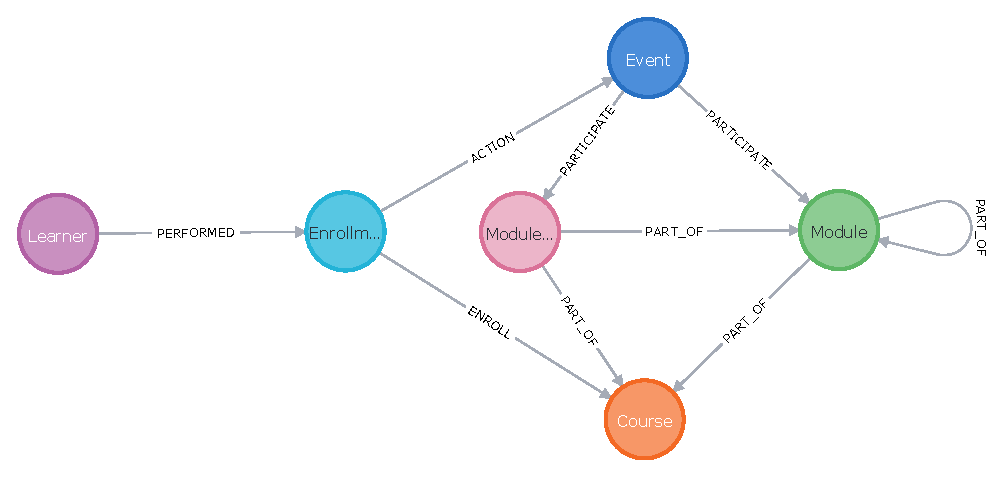
\includegraphics[width=0.45\textwidth]{assets/graph-modeling}
        }
        \caption{แบบจำลองความสัมพันธ์ของกราฟในฐานข้อมูล}
        \label{fig:graph-modeling}
    \end{figure}

    \section[method]{วิธีการดำเนินงาน}
    lorem ipsum

    \section[result]{ผลลัพธ์การดำเนินงาน}
    lorem ipsum

    \section[conclusions]{สรุปผลการศึกษา}
    lorem ipsum

    \bibliographystyle{IEEEtran}
    \bibliography{sna-ref}
\end{document}